\documentclass[journal, a4paper]{IEEEtran}

% some very useful LaTeX packages include:

%\usepackage{cite}      % Written by Donald Arseneau
                        % V1.6 and later of IEEEtran pre-defines the format
                        % of the cite.sty package \cite{} output to follow
                        % that of IEEE. Loading the cite package will
                        % result in citation numbers being automatically
                        % sorted and properly "ranged". i.e.,
                        % [1], [9], [2], [7], [5], [6]
                        % (without using cite.sty)
                        % will become:
                        % [1], [2], [5]--[7], [9] (using cite.sty)
                        % cite.sty's \cite will automatically add leading
                        % space, if needed. Use cite.sty's noadjust option
                        % (cite.sty V3.8 and later) if you want to turn this
                        % off. cite.sty is already installed on most LaTeX
                        % systems. The latest version can be obtained at:
                        % http://www.ctan.org/tex-archive/macros/latex/contrib/supported/cite/

\usepackage{graphicx}   % Written by David Carlisle and Sebastian Rahtz
                        % Required if you want graphics, photos, etc.
                        % graphicx.sty is already installed on most LaTeX
                        % systems. The latest version and documentation can
                        % be obtained at:
                        % http://www.ctan.org/tex-archive/macros/latex/required/graphics/
\usepackage{subfig}
                        % Another good source of documentation is "Using
                        % Imported Graphics in LaTeX2e" by Keith Reckdahl
                        % which can be found as esplatex.ps and epslatex.pdf
                        % at: http://www.ctan.org/tex-archive/info/

%\usepackage{psfrag}    % Written by Craig Barratt, Michael C. Grant,
                        % and David Carlisle
                        % This package allows you to substitute LaTeX
                        % commands for text in imported EPS graphic files.
                        % In this way, LaTeX symbols can be placed into
                        % graphics that have been generated by other
                        % applications. You must use latex->dvips->ps2pdf
                        % workflow (not direct pdf output from pdflatex) if
                        % you wish to use this capability because it works
                        % via some PostScript tricks. Alternatively, the
                        % graphics could be processed as separate files via
                        % psfrag and dvips, then converted to PDF for
                        % inclusion in the main file which uses pdflatex.
                        % Docs are in "The PSfrag System" by Michael C. Grant
                        % and David Carlisle. There is also some information
                        % about using psfrag in "Using Imported Graphics in
                        % LaTeX2e" by Keith Reckdahl which documents the
                        % graphicx package (see above). The psfrag package
                        % and documentation can be obtained at:
                        % http://www.ctan.org/tex-archive/macros/latex/contrib/supported/psfrag/

%\usepackage{subfigure} % Written by Steven Douglas Cochran
                        % This package makes it easy to put subfigures
                        % in your figures. i.e., "figure 1a and 1b"
                        % Docs are in "Using Imported Graphics in LaTeX2e"
                        % by Keith Reckdahl which also documents the graphicx
                        % package (see above). subfigure.sty is already
                        % installed on most LaTeX systems. The latest version
                        % and documentation can be obtained at:
                        % http://www.ctan.org/tex-archive/macros/latex/contrib/supported/subfigure/

\usepackage{url}        % Written by Donald Arseneau
                        % Provides better support for handling and breaking
                        % URLs. url.sty is already installed on most LaTeX
                        % systems. The latest version can be obtained at:
                        % http://www.ctan.org/tex-archive/macros/latex/contrib/other/misc/
                        % Read the url.sty source comments for usage information.

%\usepackage{stfloats}  % Written by Sigitas Tolusis
                        % Gives LaTeX2e the ability to do double column
                        % floats at the bottom of the page as well as the top.
                        % (e.g., "\begin{figure*}[!b]" is not normally
                        % possible in LaTeX2e). This is an invasive package
                        % which rewrites many portions of the LaTeX2e output
                        % routines. It may not work with other packages that
                        % modify the LaTeX2e output routine and/or with other
                        % versions of LaTeX. The latest version and
                        % documentation can be obtained at:
                        % http://www.ctan.org/tex-archive/macros/latex/contrib/supported/sttools/
                        % Documentation is contained in the stfloats.sty
                        % comments as well as in the presfull.pdf file.
                        % Do not use the stfloats baselinefloat ability as
                        % IEEE does not allow \baselineskip to stretch.
                        % Authors submitting work to the IEEE should note
                        % that IEEE rarely uses double column equations and
                        % that authors should try to avoid such use.
                        % Do not be tempted to use the cuted.sty or
                        % midfloat.sty package (by the same author) as IEEE
                        % does not format its papers in such ways.

\usepackage{amsmath}    % From the American Mathematical Society
                        % A popular package that provides many helpful commands
                        % for dealing with mathematics. Note that the AMSmath
                        % package sets \interdisplaylinepenalty to 10000 thus
                        % preventing page breaks from occurring within multiline
                        % equations. Use:
%\interdisplaylinepenalty=2500
                        % after loading amsmath to restore such page breaks
                        % as IEEEtran.cls normally does. amsmath.sty is already
                        % installed on most LaTeX systems. The latest version
                        % and documentation can be obtained at:
                        % http://www.ctan.org/tex-archive/macros/latex/required/amslatex/math/
\usepackage{amssymb}
%\usepackage[toc,page]{appendix}


% Other popular packages for formatting tables and equations include:

%\usepackage{array}
% Frank Mittelbach's and David Carlisle's array.sty which improves the
% LaTeX2e array and tabular environments to provide better appearances and
% additional user controls. array.sty is already installed on most systems.
% The latest version and documentation can be obtained at:
% http://www.ctan.org/tex-archive/macros/latex/required/tools/

% V1.6 of IEEEtran contains the IEEEeqnarray family of commands that can
% be used to generate multiline equations as well as matrices, tables, etc.

% Also of notable interest:
% Scott Pakin's eqparbox package for creating (automatically sized) equal
% width boxes. Available:
% http://www.ctan.org/tex-archive/macros/latex/contrib/supported/eqparbox/

% *** Do not adjust lengths that control margins, column widths, etc. ***
% *** Do not use packages that alter fonts (such as pslatex).         ***
% There should be no need to do such things with IEEEtran.cls V1.6 and later.

%Start: Das hier sorgt dafür, dass Umlaute funktionieren.
%\usepackage[main=ngerman, english]{babel}
\usepackage[main=ngerman, english]{babel}
\usepackage[utf8]{inputenc}
\usepackage{algorithm}
%\usepackage{algorithmic}
%\usepackage{amsmath}
%\usepackage{gensymb}

\usepackage{algorithm}% http://ctan.org/pkg/algorithms
\usepackage{algpseudocode}% http://ctan.org/pkg/algorithmicx
\newcommand{\var}[1]{{\ttfamily#1}}% variable

%\usepackage[hyphens]{url}
%\usepackage{hyperref}

%Ende: Das hier sorgt dafür, dass Umlaute funktionieren.
%\theoremstyle{theorem}
\newtheorem{theorem}{Theorem}[section]




% Your document starts here!
\begin{document}
	\selectlanguage{english}
	% Define document title and author
	\title{Waddle -- Waddington's epigentic landscape}
	\author{Individual report by Felicia Burtscher}
	\thanks{Special thanks go to Michael PH Stumpf, Suhail A Islam, Rowan Brackston, Ivan Croydon Veleslavov and the whole Julia community out there.}\\
	
\markboth{Imperial College: MSc Bioinformatics and Theoretical Systems Biology, \today}{}
\maketitle
%%%%%%
%WHAT I DID:
%1. literature research -- set alerts on pubmed, twitter and google search
%2. create refWorks -- for bibtex bibliograhy later
%%%%%%


% Write abstract here
\begin{abstract}
The \textit{Waddington} or \textit{epigenetic landscape} concept has become an important framework to reason about developmental processes. This project develops a set of Julia tools to determine the structure of such landscapes for a given dynamical system, as well as single cell data. We implement the probability flux method (PFM) of constructing a landscape, additionally applying kernel density estimation (KDE). Stability analysis is conducted on dynamical systems and their corresponding landscapes. In conjunction to that second, a more accurate approach %REALLY??
of the landscape is performed: Minimal Action Path (MAP) method. %The latter one has a direct interpretation to the force that would need to be applied to cross the landscape between two chosen points. %Due to computational complexity, we limited our approach to only simulate the quasi-potential given two points in space. %% IS THAT STILL TRUE?
For high dimensional systems, the topic of dimensionality reduction is addressed, with corresponding tools developed support visualisation of these high-dimensional data.
Reasonable results could be yielded for the 2-dimensional KDE as well as the PFM on the CPU; the PFM on the GPU posed a great challenge due to problems outlined in the group report and is still work in progress.


%SET SCIENTIFIC CONTEXT
%METHODS, RESULTS, CONCLUSIONS CLEAR AND PRECISE
\end{abstract}

%%----------------------------------------------------------------------------------------------------------------------------------------
%%----------------------------------------------------------------------------------------------------------------------------------------
%\section{Preface}
\section{Introduction}
The following report will focus on different methods, discussion and suggestions regarding dimensionality reduction (DR) and literature research regarding this as this was the part I was most enaged with during the project and the part that has not given enough credit in the group report (in terms of where time and brain power was speant) as it went beyond the scope and goal of our project to simulate the epigenetic landscape.
% The theory can be found in the group report
% also time on Bayesian Gaussian Latent variabel model and Hopfland, discovered together with MH
Other parts I contributed to was the Genetic Algorithm (GA) to approximate the MAP, implementing different kernels for the Kernel density estimation (KDE) in 2D, converting the MAP between two points into a quasi-potential (a now more elaborate final version has been developed), as well as different information theory approaches to the given sample data set. However, due to the very restrictive word count and to avoid overlap with the other reports this will not be the subject of the following report. For an overview we refer to the group project report, for the information theory approaches we refer to Madeleine Hall's report, for the GA as well as the KDE we refer to Lucas Ducrot's report. The final code can be found on 
%\begin{verbatim}
\textit{\url{https://github.com/burfel/waddington-project.}}
%\end{verbatim}	
%TODO: 
The \textit{README.md} will be kept self-explanatory and should give an overview of the main tools implemented. \\
Besides literature research on and the application of DR, important tasks of mine were documentation, adjusting our code, keeping our github repository nice and tidy and sharing interesting papers via a pad as literature research was a major part in the project. \\

It should be noted that in the following, I assume the reader to have read our group report. My following individual report is not technical, it is kept on a personal note and should indicate my main contributions and time spent during the research project; it reflects challenges I faced and especially learnings thereof and is therefore not a formal report.  \\

For an introduction to the Waddington's landscape and the scope of the project, we refer to the group project.

%GOAL OF PROJECT -- GOES IN GROUP REPORT
%As so much has been done already, and we did not want to reinvent the wheel, we defined our goal as follow: To develop a set of Julia tools and methods to simulate (via the Probability Flux Method (PFM), Kernel Density Estimation (KDE) and the Minimum-Action Path (MAP)) and analyse the given landscape including dynamical systems stability analysis; moreover, we wanted to provide the user with various methods to read in the data (including from sbml files), extract information from the given data set (statistical information, plots for visualisation) and based on this visualise specific genes or gene combinations after applying dimensionality reduction (DR). However, visualisation was not our focus as this has been tackled by last year's group already. 



%TODO:
%INSERT ALL REFERENCES FROM THE PAD (MAINLY SECTION LITERATURE RESEARCH), GITHUB
	

%%----------------------------------------------------------------------------------------------------------------------------------------
%%----------------------------------------------------------------------------------------------------------------------------------------
%\section{Introduction}
%
%%EXPLAIN TOPIC CLEARLY, SEE REVIEW 
%
%[SHORT INTRODUCTION TO TOPIC WILL BE GIVEN, SIMILAR TO GROUP REPORT ONE, OR ONLY REFERENCE TO GROUP PROJECT IF NO WORDS LEFT]

%%----------------------------------------------------------------------------------------------------------------------------------------
%%----------------------------------------------------------------------------------------------------------------------------------------
\section{Literature research}

%START WITH SUBSTANTIAL BACKGROUND READING

%EXPLAIN PREVIOUS WORK
%AIMS, ADVANCES CLEARLY DEFINED

Before starting with anything (except for some toy models) I did some extensive literature research on the work that has already been done regarding Waddington's landscape. This was necessary as there was no specific task given, and no underlying biological question that needed to be answered. It was probably one of the major challenges of the whole project: To find a (convincing) motivation of the project and to come up with a specific goal.\\
It is challenging to synthesise the work that has been done as very different approaches have been taken. In order to situate our work within the wider literature, we highlighted the major state-of-the-art methods that have been developed by other groups in the group report.
%I am going to highlight the major state-of-the-art methods that have been developed by other groups:
Here, I will point out the approach these methods took regarding dimensionality reduction (DR) which this report will be focusing on. 

%[UNFINISHED]

\subsection{Wanderlust}
\textit{Wanderlust} \cite{wanderlust} uses t-SNE. A non-linear method seems reasonable to apply; however, it does not consider the topography of the map when developing pseudotime orderings \cite{hopland}.

%The topography of the epigenetic landscape influences distances between cells on the 347 landscape, and therefore their effective relative positions to each other [REFERENCE]. 

\subsection{Monocle}
\textit{Monocle} \cite{monocle} uses Independent Component Analysis (ICA). This method, however, assumes a linear map, which does not seem like a realistic assumption.
%COMPARISON ICA -- PCA

\subsection{Topslam}
\textit{Topslam} \cite{topslam} uses the probabilistic Bayesian Gaussian Process Latent Variable Models (BGLVM). It can be seen as an extension of PPCA -- a probabilistic model of PCA that comes with a number of advantages.
%It extracts the relevant dimensionality of the latent embedding as well as expressing a non-linear model.

%PPCA to map the individual cells to the surface of a Waddington’s epigenetic landscape which seems like an appropriate and beneficial method to use.
%-- PLAUSIBLE, TALK ABOUT BENEFITS OF PPCA

\subsection{Hopland}
\textit{Hopland} \cite{hopland} also uses Bayesian Gaussian Process Latent Variable Models (BGLVM), it is data-driven and based on Hopfield network. 
%TALK ABOUT BGLPVM here; too complicated/ involved approach that could not be achieved within the given time frame, but might be interesting to look into in the future --> MOVE TO OUTLOOK
We investigated BGLVM a bit further but found it to be beyond the scope of this project.
For a more thorough review on the Hopland approach, we refer to Madeleine Hall's individual report.
%\subsection{Hadoop}??
%\subsection{Wishbone}?
%\subsection{SCUBA}?

%[I WILL PROVIDE AN OVERVIEW OF THE LITERATURE REVIEW THAT WILL GO INTO THE GROUP REPORT]



%%----------------------------------------------------------------------------------------------------------------------------------------
%%----------------------------------------------------------------------------------------------------------------------------------------
\section{Sample single cell data set}

%TAKE INSPIRATION FROM https://github.com/jadianes/data-science-your-way/tree/master/02-exploratory-data-analysis


%%%%-------------IN GROUP REPORT-------------
\subsection{Exploratory data analysis}

Complementary to the information given in the group report on the data (see section 5.2) that was largely taken from \cite{singlecelldata}, and the information obtained by measure-theoretic anlaysis, we provide the user with an initial exploratory data analysis. This can help the user to "get a feel" of the data set, discard outliers and serve as a starting point for a subsequent more detailed analysis. \\
The user can obtain statistics on the whole sample set, such as mean and variance of the different genes, that can be visualised or on specific genes; also more detailed statistics such as percentiles by selecting individual genes can be obtained and subsequently visualised in various manners, see proof-of-concept examples in the group report..\\

%[INSERT FIGURES HERE: MEAN, VARIANCE, BOXPLOT] 
%[INSERT TABLE HIGHEST MEAN, LOWEST MEAN, SAME FOR VARIANCE]
%BUT: OF ANY VALUE AT ALL??!

%\begin{figure}[t]
%	\includegraphics[width=8cm]{Plot}
%	\centering
%\end{figure}

%For other data analysis such as  expression of different genes over time points we refer to [REFERENCE]; a dimensionality technique will be applied in the following section. 

%such as information-theoretic approaches including mutual information (MI), for which we refer to Madeleine Hall's report. We will not discuss this any further here but refer to Madeleine Hall's individual report instead.

%The program \texttt{Readin.jl} reads in the data set; the path to the data set needs to be given as an argument. 

%%%%-------------------------------

\subsection{Feature selection}

When we visualise the Waddington's epigenetic landscape in three dimensions, typically the x-axis and y-axis correspond to the expression level of two marker genes that represent cell states, while the z-axis represents the potential. To visualise global information, both in case of real world data or simulated data based on a model of more than two genes, DR techniques would be needed (see next chapter).\\

For now, we mean to visualise the landscape with respect to two genes. For that purpose, we choose genes that have an "important" relationship and would result in a distinctive landscape. 
Additionally to computing pairwise correlations of genes, we therefore used information-theoretic approaches implemented in the \textit{InformationMeasures.jl} package to examine relationships between genes. These included eg mutual information (MI), conditional MI,  entropy and conditional entropy,%; %, interaction information, total correlation as well as partial information decomposition; 
%the program can be found on \texttt{https://github.com/burfel/waddington-project/blob/master/src/InformationMeasuresTest.jl}.\\
%This was inspired by [REFERENCE PAPER]

These methods based on information theory can be regarded as a generalisation of the ones based on statistics: They can capture non-linear relationships between variables and can handle interval and categorical data at the same time. %, and most of them are invariant to monotonic transformations of the input variables [REFERENCE].
% reference:https://arxiv.org/ftp/arxiv/papers/1403/1403.2877.pdf

% CONDIITONAL MUTUAL I
%MAXIMAL INTERACITON INFORMATION
% TOTAL CORRELATION 
%PARTIAL INFORMATION DECOMPOSITION
A summary of the results can be found in table 1 of the group report; for the plots, a discussion and further details we refer to Madeleine Hall's individual report.

%EDIT
For more on feature selection, we refer to \cite{featurelection1}, \cite{featureselection2}, \cite{featureselection3}.


%METHODS CLEAR, FOCUSED AND ROBUST.

%%----------------------------------------------------------------------------------------------------------------------------------------
%%----------------------------------------------------------------------------------------------------------------------------------------%%%%%----------GROUP REPORT------------------------
\section{Dimensionality reduction (DR)}

%This project aims to evaluate the performance of as many open source feature selection and dimensionality reduction methods as possible. The data that is going to be used will be from the Metabolomics domain.

%problem: high dimensional sample spaces, 
%(especially for applying consecutive ML algorithms)


%If the number of dimensions, ie genes in our case, is large, the number of possible states in this space grows exponentially large. In other words, with increasing dimensionality it becomes harder to sample from the space; even for a small model of three genes this can be a major challenge. Simulations take very long to run (as discussed in section ..... in the group report); 
%As DR is being applied in many different fields, 

Complementary to our motivation to apply DR outlined in the group report, DR is often used as a pre-processing step for machine learning (ML) algorithms as training on high-dimensional data sets is very time-intensive and can cause overfitting. However, no matter how universal the application of DR is, the common goal is usually the same: To reduce the complexity of the data set to a more understandable representation without losing (much) information. \\

%similarly, to train machine learning (ML) algorithms on such high-dimensional data sets is very time-intensive and can cause over-fitting. %% REFERENCE
%This problem is often referred to as \textit{Curse of dimensionality}; DR can be seen as a potential pre-processing step for machine learning algorithms.

%Therefore, it is necessary to reduce the data to fewer dimensions as a preprocessing step for ML algorithms.
% to make ML algorithms more efficient. 
%or run faster

%INTO GROUP REPORT
%In our case, the reason to apply dimensionality reduction is the purpose of visualisation. It is hard for humans to comprehend data in many dimensions. In our specific example this translates to the obvious fact that only two genes at a time (with the amplitude of the quasi-potential in a third direction) can be visualised in our 3D world, or respectively projected onto a 2D plane.\\
%
%Unlike feature selection that tries to only keep the most relevant features from the original data set, we can reduce the dimensions by applying dimensionality reduction (DR) techniques. These methods make use of the redundancy of the original data set and reduce the number of features (here: genes) by creating new linear, or non-linear, combinations of the original features.


%CHALLENGE: INTERPRETATION OF NEW FEATURES

%In the following linear as well as non-linear, including manifold learning algorithms, are presented that have (partially) been applied to our given data set in order to tackle the challenges discussed above.\\
%AAdvantages and disadvantages of different methods have been highlighted in the group report; an overview can be found in the appendix of this inidvidual report.

DR algorithms can be categorised in two main groups: Those that try to preserve the distance structure within the data (usually linear methods) and those that aim to preserve local distances over global distances (most of the manifold learning methods) \cite{umap}.\\

%TALK: Most dimensionality reduction techniques aim to find some hyperplane, which is just a higher-dimensional version of a line, to project the points onto. 

%Different methods are compared, results of the implemented functions are presented and an overall conclusion is drawn. 
%TODO
Principal Component Analysis (PCA) as a linear method and kernel PCA (KPCA) as a non-linear method have been explained in greater detail as they represent the simplest and most common, yet powerful, approaches to DR. A proof-of-concept example was presented in the group report. Methods in Julia that have been applied include KPCA, Probabilistic PCA (PPCA) and Multidimensional Scalin (MDS). However, no great insights could be gained based on the given data set and PCA seems to be a good method on the specific data set. To effectively compare the different methods more data would be needed.
%Additionally, an interesting manifold learning algorithm, Laplacian Eigenmaps (LEM), has been presented and discussed in comparison to other non-linear methods in the group report.
%in comparison to other non-linear methods.

For an overview, we categorise the main DR methods available in Julia in the diagram found in the appendix. As no good overview of the plethora of DR methods available could be found we created one on the lowest level of maths for which we refer to \texttt{https://github.com/burfel/waddington-project/tree/master/papers/dimRed}.

%for an extended explanation on all the methods we refer to [FILE ON GITHUB].


%ADD FIGURE HERE


%\subsection{Linear methods}
% theory and what implemented functions exactly do.



%%%----------------------------------------------------------------------------------------------------------------------------------------
%\subsection{Manifold learning}
%
%Non-linear DR methods also include Manifold Learning Algorithms; this it the part where a little bit of differential geometry comes into play. Certainly, manifolds are of great interest in differential geometry; for a (mathematically rigorous) definition of manifolds we refer to [REFERENCE].
%Unlike simple linear DR methods like PCA, manifold learning techniques consider the intrinsic geometry of the data; they are based on the assumption that the given data lies on an embedded non-linear manifold within the high-dimensional space. 
%Instead of projecting the data onto the "right" set of directions, we look for a manifold close to the data, project it onto that manifold and "unfold" the manifold for representation. We do this in a way that each data point is assigned a low dimensional representation while keeping its essential geometric properties such as relative distances between points unchanged.
%The data, assuming the manifold is of low enough dimension, can then be visualised in this lower-dimensional space.\\
%
%Another major difference between (most) manifold learning techniques and linear methods is that only local features of the data are considered opposed to global ones by eg taking correlations of the entire data set.\\
%
%The typical manifold learning problem is unsupervised: it learns the high-dimensional structure of the data from the data itself.%, without using predetermined classifications [REFERENCE scikit-learn]. 
%However, supervised versions exist as well.\\
%
%%https://pdfs.semanticscholar.org/333a/a1225a0364a46185aa19ec99c34b37555258.pdf
%The main problem to which different methods suggest different solutions is: How to construct a representation for the data lying on such a low dimensional manifold embedded in a high dimensional space? What are criteria for "good" and "bad" representations? %The methods presented in this project [LINK TO GITHUB FILE] will touch upon that.
%
%%The methods proposed in the following will touch upon that.
%%IThis answer should serve as a guiding question in the following.
%%% We will refer to this in the following.
%
%%two groups: 
%%- those that provide a mapping (either from high-dimensional space to low-dimensional embedding or vv); in the context of ML often views as a preliminary feature extraction step after which pattern algorithms are applied
%%- those that just give a visualisation; often based on proximity data, ie distance measurements
%
%%REFERENCE: self-organising: [Kohonen1990, Kohonen1993, Kohonen2001]
%% self-organising: They work pretty well on most contexts, very simple to understand and implrement, but lack from a solid mathematical framework (they are noc optimising any functional and they cannot be put in a statistical framework)
%

%%%%%-----------------------------from here: GOES ONTO GITHUB
%In the following, we want to give an overview of the main manifold learning algorithms applicable to our data set. However, we will keep the maths to the lowest level possible.
% In mathematics, a manifold is a topological space that locally resembles Euclidean space near each point. More precisely, each point of an n-dimensional manifold has a neighbourhood that is homeomorphic to the Euclidean space of dimension n.

%Manifold learning algorithms are implemented that way:
%All methods implemented in this package adopt the column-major convention of JuliaStats: in a data matrix, each column corresponds to a sample/observation, while each row corresponds to a feature (variable or attribute).



%%----------------------------------------------------------------------------------------------------------------------------------------
%%----------------------------------------------------------------------------------------------------------------------------------------
\section{Genetic algorithm for the Minimum Action Path (MAP)}
%[UNFINISHED]
%
%other methods discussed
%
%[REFER TO GROUP PROJECT]
%
%[PLAYING AROUND WITH DIFFERENT STARTING POINTS, BUT MAYBE LEAVE THAT UP TO [LD] AS HE WAS IN CHARGE OF IT]
%
%see \texttt{KDE\_reduction\_2D.jl}
%
%
%The GA is are a probabilistic search approach which are based on the ideas of evolution: We develop generations of solutions based on the Darwinian principle of survival of the fittest using a specific fitness function (eg an objective function in mathematical optimisation)
%
%However, because of the probabilistic development of the solution it does not guarantee (global) optimality of the solution. 
%
%% https://www.economicsnetwork.ac.uk/cheer/ch13_1/ch13_1p16.htm
%An initial population is created containing a predefined number of individuals (or solutions), each represented by a genetic string (incorporating the variable information). Each individual has an associated fitness measure, typically representing an objective value. The concept that fittest (or best) individuals in a population will produce fitter offspring is then implemented in order to reproduce the next population. Selected individuals are chosen for reproduction (or crossover) at each generation, with an appropriate mutation factor to randomly modify the genes of an individual, in order to develop the new population. The result is another set of individuals based on the original subjects leading to subsequent populations with better (min. or max.) individual fitness. Therefore, the algorithm identifies the individuals with the optimising fitness values, and those with lower fitness will naturally get discarded from the population.
%



[PSEUDOCODE]

%%----------------------------------------------------------------------------------------------------------------------------------------
%%----------------------------------------------------------------------------------------------------------------------------------------
%\section{Discussion and conclusion}

%SOME CONCRETE FACTS ABOUT KEY RESULTS. 

\section{Extended discussion}

\subsection{DR and the process over the project}\label{discussion}

As there are packages for DR available in Julia already, I was planning on comparing and evaluating different methods of DR, linear and non-linear, on a certain data set (real data and simulated data) — as performance of different algorithms heavily depend on the nature of the data — and evaluate which ones work best. 

However, as hardly any methods in \textit{MultivariateStats.jl} and \textit{ManifoldLearning.jl} were actually running (eg only two of the six manifold learning techniques), even with the help of the Julia community, my initial turned out to be over-ambitious due to the major challenges in Julia explained in \ref{label}. 
They methods have been partially flagged for fixing by the time of writing this report. Therefore, we were limited to few methods such as PCA, PPCA, KPCA and LEM and LTSA to test our given sample data set. However for the latter two, the returned objects no user recipe functions including plotting have been implemented and are therefore of no practical use. I implemented another PCA based on SVD. \\

%Due to lack of documentation, it was unclear, what the 

Two implementations of t-SNE are available in Julia [REFERENCE, REFERENCE]; none of the packages have been added to the \textit{ManifoldLearning.jl} package yet since the latest Julia fails to build them. Also, they depended on the package \textit{Gadfly.jl} that was unstable or \textit{RDatasets.jl} that was not compatible with other packages we were using at the time respectively. Also, a documentation of how to call the function needs to be added. \\

On the other hand, in Python all the major manifold learning methods are implemented and worked smoothly; also the package \textit{ScikitLearn.jl} had major flaws and even though I often did, any Python-package in Julia was recommended not to be used by some members of the community, also due to instability. \\

It should be mentioned that there was a tradeoff for me between working on DR and contributing to our actual project. 
For the first one, I could have reimplemented already existing, but broken, methods to maybe gain a better understanding for the algorithms or implemented other methods, eg the JADE algorithm for ICA or a rather involved manifold learning algorithm, such as an optimised version t-SNE. The latter was beyond the scope of our project. However, I didn’t see much point in trying to “reinvent the wheel”, and the risk that it might not work for future Julia versions if it depends on other packages was not motivating for me. %Also, we had not enough data available to test the algorithm on that would have justified an implementation; sample data sets from \textit{RDataset.jl} were difficult as the package was not compatible with \textit{DiffentialEquations.jl} and all in all, it was of little use for our actual project. 
I therefore based my understanding of the algorithms, the comparison and their benefits and drawbacks on literature as well as the implementation in Python using \textit{scikit-learn}.\\
For the second one, I was working on the other parts outlined in the introduction which went smoothly, the Julia packages were largely reliable and the code can be found in the repository. \\

Facing these major obstacles, DR (in Julia and also the theory, especially manifold learning) is an entirely different project; DR itself is an exciting research field. For comments regarding Julia, I refer to the appendix. 


\subsection{When to use which DR method?}

Following the \textit{No free lunch theorem}, there is no best method; it depends on the specific data set.
Eg Linear Discriminant Analysis (LDA) would make more sense than PCA if you have a linear classification task; however, empirical studies have shown that it is not always the case \cite{github} Although KPCA can separate concentric circles, it fails to unfold the Swiss Roll, for example; here, locally linear embedding (LLE) would be more appropriate \cite{github}. \\
As we have seen, there are various methods that generate non-linear maps, ie embedding maps of the data points to a lower dimension. Others are self-organising or based on a neural network (see \cite{hopland} presented in Madeleine Hall's individual report); the problem is usually formalised as a non-liner optimisation problem that can be solved by eg gradient descent. However, the latter only guarantees to return a local optimum; global optima are in general difficult to obtain efficiently. Also, we do not know whether the points actually lie on a manifold of lower dimension -- it's a mere assumption.
Therefore, non-linear methods that do not rely on the assumption of a low-dimensional manifold structure, such as KPCA might be more useful in some cases. 
\\
% [Quantitative Comparison of Linear and Non-Linear Dimensionality Reduction Techniques for Solar Image Archives Juan M. Banda ]
It is reasonable to say that the right DR method should be selected on the following criteria based on this priority order \cite{banda}:
\begin{enumerate}
\item Its popularity in the literature
\item The availability of a mapping function or method to map new unseen data points into the new dimensional space
\item The particular properties between the data and the type of distances between the data points (eg Euclidean vs geodesic)
\item Computational cost
\end{enumerate}

%INSERT GEODESIC/ EUCLIDEAN DISTANCE HERE
%https://arxiv.org/ftp/arxiv/papers/1403/1403.2877.pdf

To remind the reader of the difference between Euclidean and geodesic distance we added figure [REFERENCE].
\begin{figure}[H]
	\centering
	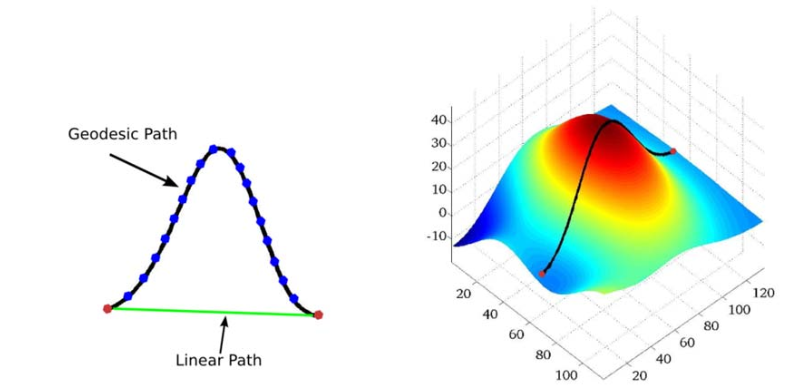
\includegraphics[width=10cm]{img/geodesic_euclidean_distance}
	\caption{Euclidean vs geodesic distance. The geodesic distance between two points is the length of the path belonging to a given manifold that joins the two points whereas the Euclidean distance is the length of the linear path between the two points \cite{euclidean}}\label{distance}
	%\centering
\end{figure}

%FIGURE: Euclidean vs geodesic distance. The geodesic distance between two points is the length of the path belonging to a given manifold that joins the two points whereas the Euclidean distance is the length of the linear path between the two points \cite{euclidean}].


Regarding popularity in the literature, %analysing the number of citations that ....
by far the most popular techniques are still classic linear techiques such as PCA or ICA -- probably due to its simplicity and intuitiveness. However, due to the non-linear nature of experimental data in many fields, we identified a trend towards applying manifold learning techniques. This might be due to the rise of non-linear experimental data in many fields and its capability of keeping the local structure of the data.

Likewise, new methods in this fields have been developed in the last two decades.



\subsection{Regarding DR also on the simulated data set}

As a group we discussed at which point in time DR should or could be applied: As we saw no way to apply DR before the actual simulation of trajectories and the estimation of landscape thereof, we could not save any computational power here. Therefore, we would treat the simulation similar to a real data set in a lower-dimensional space and motivate DR by visualisation purposes only. For where in the project of DR feeds into we refer to the workflow diagram in the group project.\\

Another challenge was the biological interpretability that has been found to be a problem elsewhere as well \cite{interpretability}. In the case of PCA, the PCs could be interpreted as linear combinations of genes as we have seen. As PCA tries to find uncorrelated variables, we could hypothesis that if there could be gene pairs identified that contribute to (always) the same PCs, they are significantly not uncorrelated, ie correlated and somehow "linked" in their expression levels. This is another way to think of the "explained variance" or information that PCA tries to preserve. With the method to identify PCs via their "barcode", they could be easily detected visually as well. Biologically, they might be controlled by the same transcription factor or occur in the same pathway, or if they have opposing "weights" in the linear combinations, ie PCs, have antagonistic effect on each other, eg one is upregulated while the other one is downregulated. By our method to identify the PCs via their barcode, we would easily track \\

%Due to the way PCA is computed these are genes that correlate positively and could eg be regulated by the same transcription factor or be found in the same pathway. 
%One could try to further investigate that experimentally. When \\

%Visualising the landscape after applying PCA makes the biological interpretation more difficult. 

On projected simulated data we could apply k-means or another clustering algorithm and compare the centroids of the cluster with the basins of attraction or fixed points from the stability analysis. 

%by a standard PCA with the basins of attraction or fixed points from the stability analysis and whether they correspond. 
We could then compute these points back into the higher-dimensional output space which would give us an idea of where approximately differentiated cell states may lie.

Still stability analysis can be done and the basins of attraction (or any other point in the lower-dimensional space) can be computed back into the original space and suggest where in the higher-dimensional input space attractor and potential differentiated cell states lie. 

% Existing algorithms are either not able to uncover the clustering structures in the data, or lose global information such as groups of clusters that are close to each other. 

\subsection{One problem of Manifold Learning techniques: Scalability}
During literature research we noticed that manifold learning isn’t widely used in papers but people seem to still rely on standard PCA and other linear DR methods, especially for single-cell data.
One reason for that might be that manifold learning techniques depend on the shape of the data, ie the mapping is implicit, and do not scale well [REFERENCE]; also computationally these methods are expensive. 
% https://arxiv.org/ftp/arxiv/papers/1403/1403.2877.pdf
One of the main problems of the manifold learning techniques explained here, is that they are only defined in a neighbourhood of the input data and they usually scale very poorly. In section [FUTURE WORKS] we refer to a recent technique that tries to solve this issue.


\subsection{Genetic Algorithm}
% https://www.economicsnetwork.ac.uk/cheer/ch13_1/ch13_1p16.htm [REFERENCE]
The GA seemed like a pretty straight forward approach and a good alternative to traditional optimisation methods.
%; especially for non-linear problem and unconstrained (or largely feasible) problems. Also, 
Eg ompared to non-linear programming models, less variables and constraints are necessary (as the variables largely depend on each other). We mainly chose the GA for its flexibility and for practical reasons to encode the action potential in the fitness function. The results we got were largly dependent on the inital population and the way we designed the mating process where we experimented a bit. 

%
%	\begin{algorithm}[t]
%		\caption{Euclid’s algorithm}\label{euclid}
%		\begin{algorithmic}[1]
%			\Procedure{Euclid}{$a,b$}\Comment{The g.c.d. of a and b}
%			\State $r\gets a\bmod b$ and \var{foobar}\label{foobar}
%			\While{$r\not=0$}\Comment{We have the answer if r is 0}
%			\State $a\gets b$
%			\State $b\gets r$
%			\State $r\gets a\bmod b$
%			\EndWhile\label{euclidendwhile}
%			\State \textbf{return} $b$\Comment{The gcd is b}
%			\EndProcedure
%		\end{algorithmic}
%	\end{algorithm}
%	In Algorithm~\ref{euclid}, variable \var{foobar} (in line~\ref{foobar}), corresponds to\ldots
%


% and the type of models that can be considered. A comparison between the non-linear programming problem and its description as a GA can be found in [REFERENCE].%[https://www.economicsnetwork.ac.uk/cheer/ch13_1/ch13_1p16.htm ].
%For a discussion of the results and problems encountered, we refer to the group report and Lucas Ducrot's individual report.

%insert pseudocode

\subsection{Different kernels in Kernel Density Estimation (KDE)} 

Other kernels implemented for the KDE in 2D including the linear kernel, cosine kernel, tophat kernel and epanechikov kernel 
have been implemented but not evaluated and compared yet.

%%----------------------------------------------------------------------------------------------------------------------------------------
%%----------------------------------------------------------------------------------------------------------------------------------------
%\section{Outlook}

%IMPLEMENT JADE ALGORITHM (WHICH I BEGAN) BUT STOPPED AS I FELT IT WAS OF NO USE FOR OUR PROJECT. 
%
%DISCUSSION AND CONLUSION, FUTURE WORK
%
%DISCUSS LITERATURE, WHY WOULD STDE BE USEFUL?
%
%CRITICALLY DISCUSS FUTURE WORK
%
%
%%%----------------------------------------------------------------------------------------------------------------------------------------
%\subsection{Manifold Learning}
%
%
%%%----------------------------------------------------------------------------------------------------------------------------------------
%\subsection{Data set}
%%if more data sets available...
%%compatible sample data set. cross-validate
%%use python tools available
%
%%%----------------------------------------------------------------------------------------------------------------------------------------
%\subsection{Genetic algorithms}
%% compare different kernel methods
%% implement other methods for optimisation problem
%
%\subsection{Fix broken functions in Julia}
%% if still not runnign in next round
%%Also a more user-friendly documentation 
%
%
%
%
%%Many issues, Many things that need fixing.
%%Often only on current master (checkout, after deleting cache), \begin{verbatim}
%%UndefVarError: <function> not defined
%%\end{verbatim}
%%was a common error message.
%%% SEE PHOTOS
%%
%%ICA -- fails to converge
%%
%%ManifoldLearning cannot be visualised
%%


\section{Future work}

\subsection{Run DR methods on multiple data sets}

Still an interesting task to do is to run different DR methods explained here, eg by using the scikit-learn methods in Python, on a large pool of data sets; for other methods available in Python that could have been useful for other parts of the project we refer to \ref{suggestionsjulia}. Provided the data is available, the easiest as fastest implementation could probably be achieved by the scikit-learn methods in Python. This way, we can get a feel for when or on what kind of data some methods work best, maybe identify emerging patters, and develop an understanding that is hard to do by just reading literature and understanding the theory. One can then come up with improvements (as there is always room for improvement), test it on sample data sets and work out the maths behind it. A good review where the different DR methods are summarised would be useful, too. Which methods to select is often not easy and highly depends on the data under study.\\

Also, comparing the running time of different methods and cross-check it with results found in literature would be worth doing.

As single cell data are often very noisy which might affect DR techniques, it might be recommendable to preprocess data using some single-cell analysis technique, eg \textit{PAGODA} [REFERENCE].


\subsection{Manifold learning}
Comparing different manifold learning algorithms seems especially interesting as it is a vibrant research field.\\

\subsubsection{MLLE}
The \textit{Modified Locally-Linear Embedding (MLLE)} algorithm has shown to be another improvement of LLE [REFERENCE] as it addresses the regularisation problem which leads to distortions in LLE maps outlined in the theory part. For that, it uses multiple weight vectors in each neighbourhood. This method would be interesting as it produces robust projections similar to Hessian LLE but without the significant additional computational cost [REFERENCE scikit-learn].
Apart from the many manifold learning method that are (currently) not working in Julia, MLLE does not yet exist in Julia and might be a suggestion to implement in the future.\\


\subsubsection{Ricci Flow in case of different curvature} 
We have seen that the standard Manifold Learning algorithms bear the assumption that the local neighbourhood of a point in the high-dimensional space is roughly equal to the tangent space at that point. Even if the neighbourhoods of points on the manifold have very different (Gaussian) curvature, they would still be treated equally and projected down to the lower-dimensional space in the same way. However, as this often is the case, standard DR are poorly locality-preserving. [REFERENCE] suggests a solution to this: We can perform an operation on the higher-dimensional space using Ricci flow before applying manifold DR. With Ricci Flow we transform each local neighbourhood of the higher-dimensional manifold to a patch with constant curvature. Then, the higher-dimensional manifold as a whole is transformed to a subset of a sphere with constant positive curvature. They could show that this method outperforms other manifold learning algorithms with better neighbourhood preserving rate.% https://arxiv.org/pdf/1703.10675.pdf [MAYBE PICTURE FROM RICCI PAPER HERE]

[MAYBE INSERT FIGURE FROM PAPER]


\subsubsection{Scalability}

%Also, the maths can be deterring sometimes. 
Manifold learning in scikit-learn have proven to be good and there is also a scalable CPU-bound manifold learning package available in Python (\textit{Megaman}). However, especially for the application on single-cell data, better manifolds learning methods need  that improve scalability and reduce the computational cost need to be developed. The Neural networks/ deep generative models approaches mentioned in the literature research section, especially \textit{scvis} in \ref{neuralnetworks} and also \textit{scVI} in \ref{deepgenmodels} are highly interesting and might replace the state-of-the art method t-SNE soon. Other methods based on neural networks hat are scalable in terms of training when using GPU are being developed.
\\ %EXPORT IF NO WORDS
Another interesting and novel manifold learning technique, not yet applied to single-cell data, found recently is the \textit{Uniform Manifold Approximation and Projection (UMAP)} on [https://arxiv.org/pdf/1802.03426.pdf]. Mathematically more involved as it draws from techniques in algebraic topology and Riemannian geometry, it scales incredibly well. It is superior to the wildly-used t-SNE in terms of visualisation quality, preserves more of the global structure and runs faster. With reference to [https://arxiv.org/pdf/1802.03426.pdf] its running time is indeed astonishing. It is also widely applicable as it makes no restrictions regarding embedding dimension. If it could be implemented to run on a GPU even, the running time would massively increase even more. This project holds great potential and could be applied to a any type of data set, including biological data.


\subsection{Genetic Algorithm}

One might look into other methods to compute th MAP such as simulated annealing or other evolutionary algorithms..


Other evolutionary algorithms, simulated annealing or divide and conquer techniques could be worth looking into. In the end, there is a no free launch theorem. Also for other metaheuristics, it is the design of that algorithm that determines their performance. And even though the results were not optimal, the GA suited our purpose well.


\subsection{Further work on Julia}

If one wants to contribute to the Julia community, one could update outdated documentations and make them more user-friendly; also many methods need bug fixing, see challenges explained in \ref{personalchallenges}. 

Apart from MLLE, a rather low hanging fruit would be to implement another ICA method based on the JADE algorithm in Julia or fix the existing one (which fails to converge on our data set) [REFERENCE]; this did not seem any relevant for our project.


\section{Conclusion}
For a general conclusion regarding the project, we refer to the group report. A personal conclusion can be found in the appendix [FIRST SECTION OF APPENDIX]..

\newpage
\appendix 

\subsection{Personal motivation and conclusion}\label{personalconclusion}
\textbf{Why Dimensionality Reduction?}\\
The high-dimensionality of the problem, especially in the real data set, was an initial motivation to apply dimensionality reduction to save computational power but especially in order to visualise data. %and save , %less for simulation purposes.
My interest in applying DR in the project stemmed the fact that I have hardly worked with it before this project but I was excited about immersing myself in the research in this field. As I had similar projects on simulations in the past, I wasn’t exactly excited about the simulation (PFM) part and the effort to get it running on a GPU in CUDA. My C skills aren’t that great and I believe things could have been implemented easier and faster if we used CuPy [REFERENCE] and our project was based on Python; I think, initialising kernels in CUDA can be a lot of work and I would say not state-of-the-art anymore; there are more convenient tools available. 
\\
\textbf{Why so much literature research?}
I was predominantly looking for an interesting research question that we could try to answer or maths that got me “hooked”. Also, I wanted to do read the relevant literature (and ask communities) that explain these methods and their advantages and/or disadvantages to first gain an understanding of which methods are appropriate. Also, especially some manifold learning algorithms are rather involved (mathematically).
\\
\textbf{Personal conclusion: }
I saw this project and the great part of literature research to it as a learning project. I learned how to use and tried to understand Julia; however, I wouldn’t use Julia as it is now again for a bigger project where the main purpose is not to contribute to the community; for this project the programming language was a great limitation.
The project’s code is solely written Julia (except the C parts in CUDA) and we developed something new regarding Waddington’s landscape. I encountered an exciting research field (DR), some interesting papers and ideas for future projects (see [REFERENCE]).


%%----------------------------------------------------------------------------------------------------------------------------------------
%%----------------------------------------------------------------------------------------------------------------------------------------
\section{(Personal) challenges and comments}\label{personalchallenges}


%%----------------------------------------------------------------------------------------------------------------------------------------
\subsection{Motivation}
As already outlined, one of the main challenges for me was the fact that we were lacking a clear motivation for the project; there was no real (biological) question we were trying to be asnwered. The more literature research we did and encounters solutions like \textit{Netland}, \textit{Hopland} and \textit{topslam}, the less motivating and harder it got to come up with something "novel". This might sound similar to the development many people undergo during their PhD and is probably a major part of research; for me, it was unlike previous projects and I took it as part of the learning process.
However, we can claim that we are the first group to produce something in Julia and we finally did achieve to accomodate our work and situate it in the wider literature. 

%%----------------------------------------------------------------------------------------------------------------------------------------
\subsection{Julia}\label{julia}
Julia and the contribution to the Julia community, to produce something that would actually be used, was my main motivation for the project. Unfortunately, Julia turned out to be a major drawback to our work, and to my part especially.

%%-----------------------------------------------------------------
\subsubsection{High volatility}
Julia is still a teenager and therefore unstable; version 1 isn't out yet. The volatility, especially in light of the probably soon to be published version 0.7
caused methods in packages to run at some points of the project (see \ref{discussion}). %; eg out of the six methods in \textit{ManifoldLearning.jl} only one actually worked. 
However, this is only a snapshot of the current situation; people keep chaging, moving and renaming methods which makes it very likely that our code needs fixing at some later point in time as well. Attention to bug fixing is 
Also the Julia community, even though very responsive especially on \textit{https://discourse.julialang.org/} including developers, refer to the instability of the packages themselves and could therefore be of limited help. %to which they weren't able to be much of help to me/us either. 
This meant, I had to redefine my initial goal of comparing differnent DR methods on the data set.
In another programming language such as Python this would have not been the case, as eg [REFERENCE PACKAGE SCIKITLEARN] contains ready-to-be-used stable functions of most of the major DR algorithms; however, using these would have been contrary to our actual goal to develop something in Julia.
%see methods that have been implemented in Python, scilearn.

%%-------------------------------------------------------------------
\subsubsection{Conflicts between packages}
Conflicts between packages like \textit{DifferentialEuqations.jl}, \textit{MultivariateStats.jl}, \text{Gadfly.jl} to only name a few was probably the biggest time-consuming aspect; packages needed to be checked out, added, pulled from the master, cleared from the cache over and over again; workarounds needed to be found. 
% and one could develop an expertise just in that to an extent that it wasn't much fun to work with anymore. 
%loading packages did take a while
% left me frustrated, motivation down.
However, here the julia community could sometimes help out.
Additionally, precompiling packages was a major time-consuming aspect. All in all, Julia's good performance comes at a very high price.

%%---------------------------------------------------------------------
\subsubsection{Documentation}
% documentation
As the documentation of specific packages including \textit{MultivariateStats.jl} and \textit{ManifoldLearning.jl} are very sparse and to large extent deprecated, it was a challenging to not only get things running but also to understand the implementation including accessible properties of the methods. The excellent documentation for data types and standard packages can serve as a model. \\
%FUTURE WORK: good documentation


\subsection{Suggestions regarding Julia}\label{suggestionsjulia}
%To draw a conclusion to that, 
Having mentioned all the challenges with Julia, I would like to stress that I am not trying to downplay Julia. \\

Julia has potential and is an exciting, intuitive and promising language to contribute to and I feel our work can be seen as an investment. I like that it's open-source and all available on GitHub. Julia can even be fun to code in (once all necessary packages have been installed and you have learned how to decipher her error messages). Also, for developing single packages/ functionalities it is suitable. However, for a rather big research project that depends on multiple (unstable) packages, I question its practicability.
Clearly, using Python for the project would have made life easier; also, only considering the time constraint, I would have been more reasonable to stick with Python. The community is large, the language stable, documentation great and many tools are available. 
Having said that, I will certainly keep monitoring it as it is further developed and improved. \\


I can see why people get excited Julia. It is an easy language, has good support for functional programming and its raw speed is close to those of a compiled language like C convincingly presented in the cross language validation on \textit{http://julialang.org/}. 
%Python and other high level languages seem to be far behind in term of speed. 
However, I was asking myself how these Python benchmarks were written -- probably in native Python and not in an optimised version. It might be more insightful to compare the performance based on tasks and once experts in the specific languages have produced the best code they can to perform these tasks. Indeed, as shown in [REFERENCE] it is possible to achieve the same benchmarks when one uses Python better and its tools. This is supported by the running time analysis regarding the simulation on the GPU (see group report).
In fact, I think it is less of a question of whether to use Python, C or Julia but the major difference can be achieved by GPU instead of CPU.\\
Still, there are plenty of tools available to optimise Python including \textit{numpy} based on C or the C extension \textit{Cython}, \textit{Numba} that contains high performance functions written directly in Python and also \textit{CuPy} (a NumPy-like API accelerated with CUDA) which could have been used for simulation. The latter might also be handy to run some computations, eg DR methods on different data sets, and compare them to get a feel and start to understand rather than relying on one's understanding from reading literature. One might also try to use Numpy/Scipy with Intel MKL and Intel Compilers to optimise Python code; but often it is already enough to write critical parts in Cython.\\
\textit{PyTorch} as an machine learning library for Python that also runs on the GPU might have been useful to get manifold learning algorithms in \textit{scikitlearn} onto a GPU. PyTorch already optimises standard optimisation algorithms.  \\

As things move very fast in this field that it is almost hard to keep up, and given the enormous brain power including money from companies that are behind tools like \textit{PyTorch} and also \textit{TensorFlow}, the numerus libraries that are available in Python, it is very unlikely that a few Julia developers will outcompete the developments currently happening in Python. \\

In the end, the optimisation achieved by Julia does not seem very relevant to me; however, it can be a language fun to play around with.

%[REFERENCE] https://www.ibm.com/developerworks/community/blogs/jfp/entry/Python_Meets_Julia_Micro_Performance?lang=en



\subsection{\textbf{On a personal note -- reflection and learnings}}

%%----------------------------------------------------------------------------------------------------------------------------------------
%%----------------------------------------------------------------------------------------------------------------------------------------
%\section{On a personal note -- learnings, comments, feedback } % with humour

 % with humour

The following part is a reflection on learnings that will be useful for the projects to follow and especially other group or open-source projects in the future.\\

%\subsubsection{Project Management skills}

Working in a group can often be challenging but also a great opportunity to develop soft skills useful elsewhere in life. Over the course of the project, I could develop project management skills and I found it great to work in a diverse team, with people from different disciplines. \\
We had to establish means of communication (between group members as well as group and supervisor). Since we were locally close to each other most of the time, a pad (\textit{\url{http://pad.spline.de/}}), emails and a messaging app were sufficient for exchanging ideas including sharing links to interesting papers.

\subsection{My top 7 learnings:}

The plan was “to look before we dived deep”. We wanted to get a feel of what's already "out there", and whether our ideas have been previously approached. Literature research can sometimes be overwhelming, as there are not only many papers but also software repository such as \textit{GitHub} or \textit{SourceForge} available. As often engaging with the network of researchers in the field can be invaluable, we also tried to contact authors when we found code that was not running (eg Matlab code in [REFERENCE Hopfield paper].

%and also demotivating
%at some point we needed to start,

\hfill
\subsubsection{Learning \#0: Get all the set-up done quickly}
Install or ask to have all software installed right from the beginning; this saves emails and time. Also make sure that the computer is sufficiently fast, if not, find out why not, and the graphics okay (the editor \textit{Atom} often seemed to be sluggish) or switch to a laptop. Make sure you can access the computer from remote, so you can work independently.

\hfill
\subsubsection{Learning \#1: Divide tasks and define interfaces clearly}
Even though we could not clearly define functionalities required and interfaces (input/output) between certain components of the work from the beginning, we did manage to split work to explore different parts of the project early-on. However, some of us carried our “exploratory phase” (toy models, literature research etc) until very far into the project, kept brainstorming ideas and adjusting (individual) goals as we went along; this might have been largely due to the fact that we could not start off with a clear-defined goal and our work wasn’t based on a specific paper. \\
Regular meetings to discuss progress and inform other group members about one’s work and keep everyone in the loop was proven to be useful. 

\hfill
\subsubsection{Learning \#2: Always pull and push}
We chose \textit{GitHub} as a version control repository to share, backup and edit each other’s code as well as \textit{overleaf} to work on the report; our final code can be found on \textit{https://github.com/burfel/waddington-project}. One take-away from working with GitHub, especially when working on one single branch, is: \textit{Always pull first and push regularly!} This cannot be stressed enough. This avoids time-consuming merging phases and avoid double-work which often happened as we were working on the same code at the same time. 
Personally, I am strongly in favour of an open approach of sharing source code as I hold this to be important for an sustainable future in science; too often results cannot be reproduced when the code isn’t reviewed or even shared.

\hfill
\subsubsection{Learning \#3: Comment code}
Commenting code is especially necessary when working together on code. Not only for documentation reasons for users or developers to build upon your code but also to make it understandable to you and “why” you implemented it that way — as one wise man once said to me: “Each line of comment is a conversation between you and your future self”. Also using meaningful variable names and formatting the code consistently can have great benefits.\\
Understanding other people’s (uncommented) code often takes more time than starting from scratch — a major problem in industry that has recently been addressed by a startup from Imperial (\textit{Codeplot}); commenting therefore prevents time drains and errors. However, comprehending commented and readable code can be enriching and help you develop empathy as well. In the end, \textit{writing code is like writing poetry}. 
I had to learn this lesson in the past the hard way
%and too often I started off from scratch because other people’s code was not readable or very unintuitive for me; 
%and I made myself in charge of making sure that also my team members stick to that rule.
and was trying to get my team members stick to that rule as well. 


\hfill
\subsubsection{Learning \#4: Do not get lost in literature research, keep track of your readings}
This might especially be a personal learning. Constant alerts by \textit{Google scholar} and \textit{pubmed} were constantly throwing me back into reading mode, even during the implementation part, but most of the time not relevant. It is easy to get dragged away and find things you might be more interested in working on (eg topological data analysis tools are interesting but only remotely relevant for our 10-week project), especially if you lack a clear-defined goal. Literature research often can be overwhelming. Therefore, it is good to find a way how to best keep track of the readings and resources and tools used for literature research; otherwise, it can make the write-up especially painful. %I learnt this too late.

\hfill
\subsubsection{Learning \#5: Keep track of your achievements/ problems/ ideas}
Also, to reflect weekly on the work like writing down your weekly achievements and problems and ideas and steps for the following week, seems like a motivating and useful thing to do. This might help you to refocus and prevent to go overboard with the reading (see learning \#5) and fits my big-picture thinking. Also, it might prevent you from jumping between tasks too much. Setting milestones for oneself or the group might be useful too. 

\hfill
\subsubsection{Learning \#6: Don't procrastinate}
You can start your report early; don't leave things until the last minute. Mabye that's just something for (active) procrastinators like me.

\hfill
Maybe these top learning are not only useful for me but for someone else as well (as report from previous year's seemed to be shared sometimes).

%%----------------------------------------------------------------------------------------------------------------------------------------
%%----------------------------------------------------------------------------------------------------------------------------------------
% Now we need a bibliography:
\begin{thebibliography}{99}
	
	\bibitem{waddington}
	Waddington CH. \textit{The Strategy of the Genes}. Routledge, 2014. First published in 1957. 
	
	\bibitem{singlecelldata}
	Stumpf PS, Smith RCG, Lenz M, Schuppert A, M{\"u}ller FJ, Babtie A,
	Chan TE, Stumpf MPH, Please CP, Howison SD, Arai F, MacArthur BD. \textit{Stem Cell Differentiation as a Non-Markov Stochastic Process}. Cell Systems Volume 5, Issue 3, p268-282.e7, 27 September 2017 
	
	\bibitem{informationmeasures.jl}
	Chan TE, Stumpf MPH, Babtie A. \textit{Gene Regulatory Network Inference from Single-Cell Data Using Multivariate Information Measures}. Cell Systems Volume 5, Issue 3, p251-267.e3, 27 September 2017.
	
	\bibitem{infotheo}
	Jenkinson G et al. \textit{Potential energy landscapes identify the information-theoretic nature of the epigenome}.
	Nature Genetics 49, 719-729, 2017.
	
	\bibitem{scikit}
	scikit-learn. \textit{https://plot.ly/ipython-notebooks/principal-component-analysis/}, 15 March 2018.
	
%	\bibitem{lala}
%	SEE PAPERS ON PAD ADN GITHUB.
%	
	
	%%%%-----DR methods
	
	\bibitem{ricci}
	Li Y and Lu R. \textit{Applying Ricci Flow to High Dimensional Manifold Learning}.
	arXiv:1703.10675v4, 26 March 2018.
		
	\bibitem{zifa}
	Pierson E and Yau C. \textit{ZIFA: Dimensionality reduction for zero-inflated single-cell gene expression analysis}.
	Genome Biology, 16:241, 2015.
	
	\bibitem{scvi}
	Lopez R et al. \textit{A deep generative model for gene expression profiles from single-cell RNA sequencing.}
	arXiv:1709.02082v4, 16 January 2018
	
	\bibitem{zinb-vae}
	Lopez R et al. \textit{A deep generative model for gene expression profiles from single-cell RNA sequencing}.
	arXiv:1709.02082v1, 7 September 2017.
	
	\bibitem{zifa-url}
	https://github.com/epierson9/ZIFA, 27 February 2018.
	
	\bibitem{deepgenmodels}
	Ding J, Condon AE, Shah SP. \textit{Interpretable dimensionality reduction of single cell transcriptome data with deep generative models}.
	https://www.biorxiv.org/content/early/2017/09/01/178624, 1 September 2017.
	
	\bibitem{neuralnetworks}
	Lin C et al. \text{Using neural networks for reducing the dimensions of single-cell RNA-Seq data}. %%GOOD READ!!!!
	Nucleic Acids Research, Volume 45, Issue 17, 29 September 2017.
	
	\bibitem{interpretability}
	Ding J, Condon A and Shah SP. \textit{Interpretable dimensionality reduction of single cell transcriptome data with deep generative models}.
	http://dx.doi.org/10.1101/178624, 1 September 2018.
	
	%\bibitem{autoencoder}
	
	\bibitem{umap}
	McInnes L and Healy J. \textit{UMAP: Uniform Manifold Approximation and Projection for Dimension Reduction}.
	arXiv:1802.03426v1, 9 February 2018.
	
	\bibitem{scater}
	McCarthy D and Wills QF. \textit{Scater: pre-processing, quality control, normalization and visualization of single-cell RNA-seq data in R}.
	Bioinformatics, 33(8), 2017, 1179-1186, 14 January 2017.
	
	\bibitem{bioconductor}
	Bioconductor. \textit{https://www.bioconductor.org/help/course-materials/2017/BioC2017/Day2/Workshops/singleCell/doc/workshop.html}, 25 March 2018.
	
	%%%------on DR---------------------
	
	\bibitem{featureselection}
	Debahuti M et al. \textit{Feature Selection in Gene Expression Data Using Principal Component Analysis and Rough Set Theory}.
	Software Tools and Algorithms for Biological Systems, pp 91-100, 15 March 2011.
	
	\bibitem{featurelection1}
	Dash M and Liu H. \textit{Feature selection for classification}.
	Intelligent Data Analysis, Volume 1, Issues 1-4, 1997.
	
	\bibitem{featureselection2}
	Guyon I and Elisseeff A. \textit{An Introduction to Variable and Feature Selection}.
	Journal of Machine Learning Research 3, 2003.
	
	\bibitem{featureselection3}
	Saeys Y, Inza I and Larranaga P. \textit{A review of feature selection techniques in bioinformatics}.
	Bioinformatics, Colume 23, Issue 19, 1 October 2007.

	
	
	%%%%-----on epigenetic landscape-----
		
	\bibitem{bifurcation}
	Marco E et al. \textit{Bifurcation analysis of single-cell gene expression data reveals epigenetic landscape}.
	PNAS, https://doi.org/10.1073/pnas.1408993111, 30 December 2014.
	
	\bibitem{bistability}
	Ferrell JE. \textit{Bistability, Bifurcations, and Waddington's Epigenetic Landscape}.
	Current Biology, Volume 22, Issue 11, 5 June 2012.
	
	\bibitem{myogen}.
	Asp P et al. \textit{Genome-wide remodeling of the epigenetic landscape during myogenetic differentiation}.
	PNAS, https://doi.org/10.1073/pnas.1102223108, 31 May 2011.
	
	\bibitem{addiction}
	Maze I and Nestler EJ. \textit{The epigenetic landscape of addiction}.
	Annals of the New York Academy of Sciences, https://doi.org/10.1111/j.1749-6632.2010.05893.x, 27 January 2011.
	
	\bibitem{alzheimer}
	Lord J and Cruchaga C. \textit{The epigenetic landscape of Alzheimer's disease}.
	Nature Neuroscience, Volume 17, Numer 9, September 2014.
	
	\bibitem{renalcancer}
	Morris MR and Latif F. \textit{The epigenetic landscape of renal cancer}.
	Nature reviews Nephrology 13, 47-60, 2017.
	
	
	%%%%----models-----
	
	\bibitem{hopland}
	Guo J and Zheng J. \textit{HopLand: single-cell pseudotime recovery using continuous Hopfield netowrk-based modeling of Waddington's epigenetic landscape}.
	Bioinformatics, Volume 33, Issue 14, 15 July 2017.
	
	\bibitem{wanderlust}
	Bendall SC et al. \textit{Single-cell Trajectory Detection Uncovers Progression and Regulatory Coordination in Human B Cell Development}.
	Cell, Volume 157, Issue 3, 24 April 2014.
	
	\bibitem{topslam}
	Zwiesele M and Lawrence ND. \textit{Topslam: Waddington Landscape Recovery for Single Cell Experiments}.
	bioRxiv, https://doi.org/10.1101/057778, 8 June 2016.
	
	\bibitem{wishbone}
	Setty M et al. \textit{Wishbone identifies bifurcating developmental trajectories from single-cell data}.
	Nature Biotechnology 34, 637-645, 2016.
	
	\bibitem{diffusionmaps}
	Haghverdi L, Buettner F and Theis FJ. \textit{Diffusion maps for high-dimensional single-cell analysis of differentiation data}.
	Bioinformatics, Volume 31, Issue 18, 15 September 2015.
	
	\bibitem{netland}
	https://github.com/NetLand-NTU/NetLand
	
	\bibitem{monocle}
	Trapnell C et al. \textit{The dynamics and regulators of cell fate decisions are revealed by pseudotemporal ordering of single cells}.
	Nature Biotechnology 32, 381-386, 2014.
	
	\bibitem{scuba}
	SCUBA.
	\textit{https://omictools.com/single-cell-clustering-using-bifurcation-analysis-tool, 25 February 2018.}
	
	\bibitem{scikit-learn}
	Scikit-learn.
	\textit{http://scikit-learn.org/stable/modules/manifold.html}, 25 March 2018.
	
	\bibitem{github}
	\textit{https://github.com/rasbt/python-machine-learning-book/blob/master/faq/dimensionality-reduction.md}, 25 March 2018.
	
	\bibitem{banda}
	Banda JM, Angryk RA, Martens PC. \textit{Quantitative Comparison of Linear and Non-linear Dimensionality Reduction Techniques for Solar Image Archives}.
	25th International FLAIRS Conference, 16 May 2012.
	
	\bibitem{euclidean}
	Sorzano COS, Vargas J and Pascual-Montano A. \textit{A survey of dimensionality reduction techniques}.
	\textit{https://arxiv.org/ftp/arxiv/papers/1403/1403.2877.pdf}
	
	\bibitem{megaman}
	Megaman.
	\textit{https://github.com/mmp2/megaman}, 25 March 2018.
	
	\bibitem{cupy}
	CuPy.
	\textit{https://github.com/cupy/cupy}, 25 March 2018.
	
	\bibitem{numba}
	Numba.
	\textit{https://numba.pydata.org/}, 25 March 2018.

	\bibitem{cython}
	Cython.
	\textit{http://cython.org/}, 25 March 2018
	
	\bibitem{overview}
	Veys S. \textit{A comparative review of dimensionality reduction methods for high throughput single-cell transcriptomics}
	Universiteit Gent, 2016.

	
	%https://www.ibm.com/developerworks/community/blogs/jfp/entry/Python_Meets_Julia_Micro_Performance?lang=en

%%%-------OVERVIEWS ON DIMRED--------
% https://arxiv.org/ftp/arxiv/papers/1403/1403.2877.pdf
	
	
\end{thebibliography}

% Your document ends here!
\end{document}
